\section{Simulation}
\label{simulation}
\nomenclature{DOF}{Degree of freedom}
A 6-DOF flight simulator was used to validate the drag prediction method before hardware was purchased. The main utility of the simulator was to provide simulated flight test data with signals that contained no errors. The actual sensors used for flight testing contain noise, and this noise can be added onto the pure simulator signals to test the sensitivity of the drag polar regression to sensor accuracy.

\subsection*{Simulation Environment}
The flight simulator used was a model of the de Haviland Beaver that comes as a demo in the Aerospace Toolbox of Simulink. The Simulink model was modified to output required signals to the workspace, which essentially created a sensor with zero noise. The mass, moments of inertia, and reference lengths were then scaled to those of a Zagi R/C aircraft\cite{stevens2003aircraft}. The original Simulink model was already connected to a FlightGear Flight Sim, used as a visualization engine. This model was slightly altered to make flight gauges function properly.

\subsection*{Simulation Inputs}
The engine forces and moments were set to zero in the simulator, to match the assumption of a folding propeller.
The drag force calculation built into the Beaver Simulink model was replaced with a parabolic drag polar of the form

\begin{align}
C_D &= C_{D_0} + K_1(C_L(\alpha)-C_{L_{min}})^2+\frac{(C_L(\alpha))^2}{\pi eAR}
\end{align}
\nomenclature{$AR$}{Aspect ratio}
\nomenclature{$C_L$}{Lift coefficient}
\nomenclature{$C_D$}{Drag coefficient}
\nomenclature{e}{Wing lift distribution}
\nomenclature{$C_{D_0}$}{Parasite drag coefficient}

%todo:redo simulation to match this. Also, propagate noise properly and match sensors. and cite NACA 4412 data
Airfoil data, including $K_1$, $C_{L_{min}}$, and $C_L(\alpha)$, was taken from nonlinear aerodynamic data of a NACA 4412. While this approximation to a drag polar does not capture the nonlinear section of profile drag rise due to stall, it does represent the limited lifting capability of a real wing, making it more realistic than assuming the wing does not stall.
\subsection*{Simulation Results}
The first goal of the simulation testing was a to verify the drag polar equations were correct, and that the data analysis routines developed in MATLAB did in fact match inputs to outputs. The simulation was initialized with various initial states to ensure there was no dependency on initial conditions. The vehicle was then flown by an R/C aircraft pilot using a joystick attached to the simulation. It was noted early in the simulation testing that flying a sweep of speeds was beneficial, as a wider range of the drag polar was flown. This result was included in much of the flight test planning. After adequate data had been taken, the data was analyzed without adding simulated sensor noise. The results are shown in Figure \ref{dragPolarNoNoise}.

\begin{figure}[H]
  \centering
  
    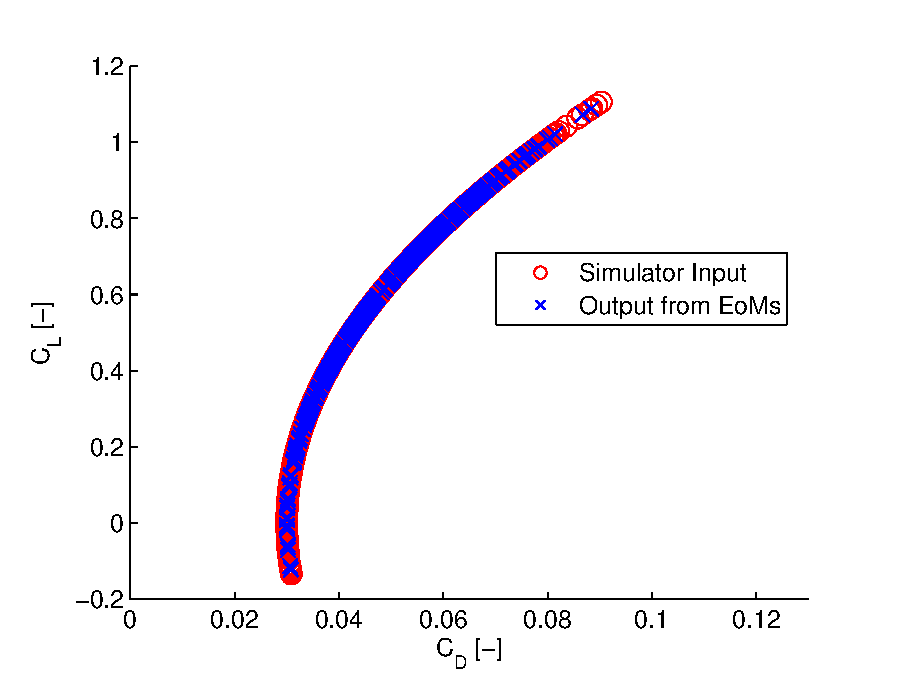
\includegraphics[width=0.5\textwidth]{figures/dragPolarNoNoise.eps}
    \label{dragPolarNoNoise}
    \caption{Data Analysis Verification (No Noise)} 
\end{figure}

Figure \ref{dragPolarNoNoise} shows that the equations of motion used in the data analysis functions properly calculate the coefficients being passed into the system. With this result, noise was added to the system to see how sensitive coefficient estimation was to noise in each sensor. This process was a balancing act between available sensor accuracy and the desired accuracy of the final solution. The final result guided sensor selection to those discussed in Section \ref{hardware}. To check if the final sensors chosen were acceptable, Gaussian noise was added to each state, with a mean of zero and a standard deviation equal to the root-mean-squared error listed in the manufacturer's data sheet for each sensor.
\begin{figure}[H]

  \centering
    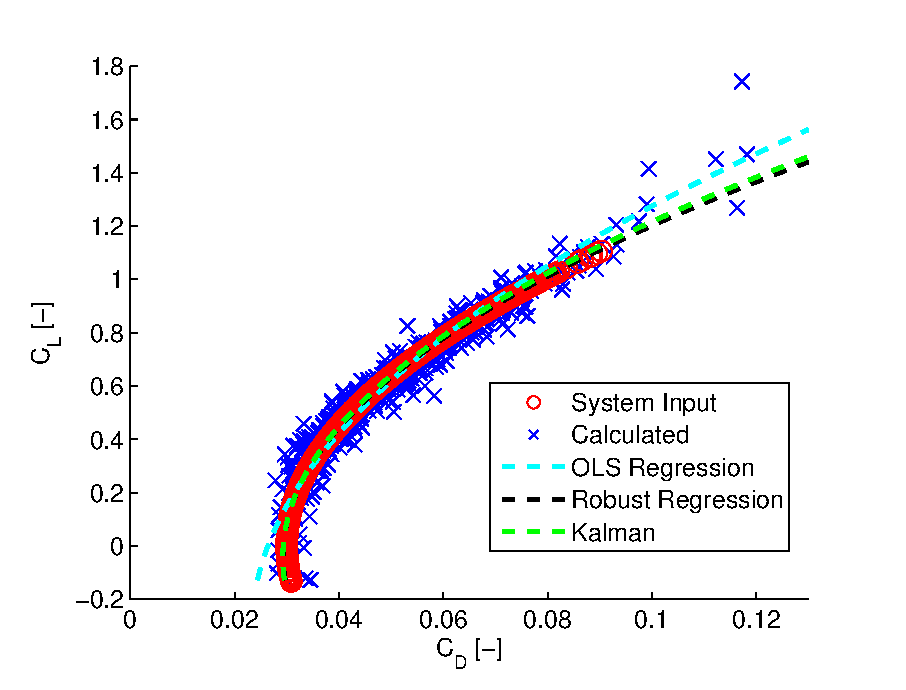
\includegraphics[width=0.5\textwidth]{figures/simDragPolarNoise.eps}
      \caption{Drag Polar Prediction of Simulated Test Flight} \label{dragPolarNoise}
\end{figure}

%todo:redo the simulation with new sensors and update table. also update drag polar to be all 3 components. and update airfoil data
For the particular simulated test flight shown in Figure \ref{dragPolarNoise}, the estimated drag polar coefficients had error coefficients outlined in Table \ref{simCoeffErrorTable}.

\begin{table}[ht]
\caption{Nonlinear Model Results} % title of Table
\centering % used for centering table
\begin{tabular}{c c c c} % centered columns (4 columns)
\hline\hline %inserts double horizontal lines
 & $C_{D_0}$ & $K_1$ & $K_2$ \\ [0.5ex] % inserts table 
%heading
\hline % inserts single horizontal line
System Inputs & 0.0493 & 0 & 0.03 \\ % inserting body of the table
OLS Estimate & 0.0355 & -0.0136 & 0.02927 \\
Robust LS Estimate & 0.0460 & -0.0037 & 0.0292 \\ [1ex] % [1ex] adds vertical space
\hline %inserts single line
\end{tabular}
\label{simCoeffErrorTable} % is used to refer this table in the text
\end{table}
\nomenclature{OLS}{Ordinary least squares}
The results of this simulated flight test showed that the measurement system outlined in Section \ref{hardware} predicted the simulated drag polar with a reasonable error. It also demonstrates the necessity of the heteroskedasticity correction, as the OLS regression has a 38\% error on $K_2$ and a 9\% error on $C_{D_0}$, while the robust regression has a 7\% error on $K_2$ and a 3\% error on $C_{D_0}$.